\section{Results}\label{sec:results}

\subsection{Base case calculation}
As a reference for all following calculations, a model representing the final design of the Blennerhassett Island Bridge is investigated. The results obtained by the calculations are then compared to the ones in the design drawings for plausibility. A particular challenge is the determination of the self-equilibrium stress state. As the arch was defined as an unsuitable parabola, appropriate hanger forces were determined by trial and error in the design. These permanent hanger forces of the final design are available in the drawings. However, for the calculation of the base case they are unsuitable, as the load distribution in the model is simplified. Instead of another trial and error procedure for the base case, the hanger forces are obtained as the result of a simultaneous arch and tie moment optimisation. Thereby, the moment in the arch is weighed by a factor of 1.5 in order to achieve on optimal similarity. The internal force distributions for the permanent state are shown in Fig. [].of the base

\begin{figure}
    \centering
    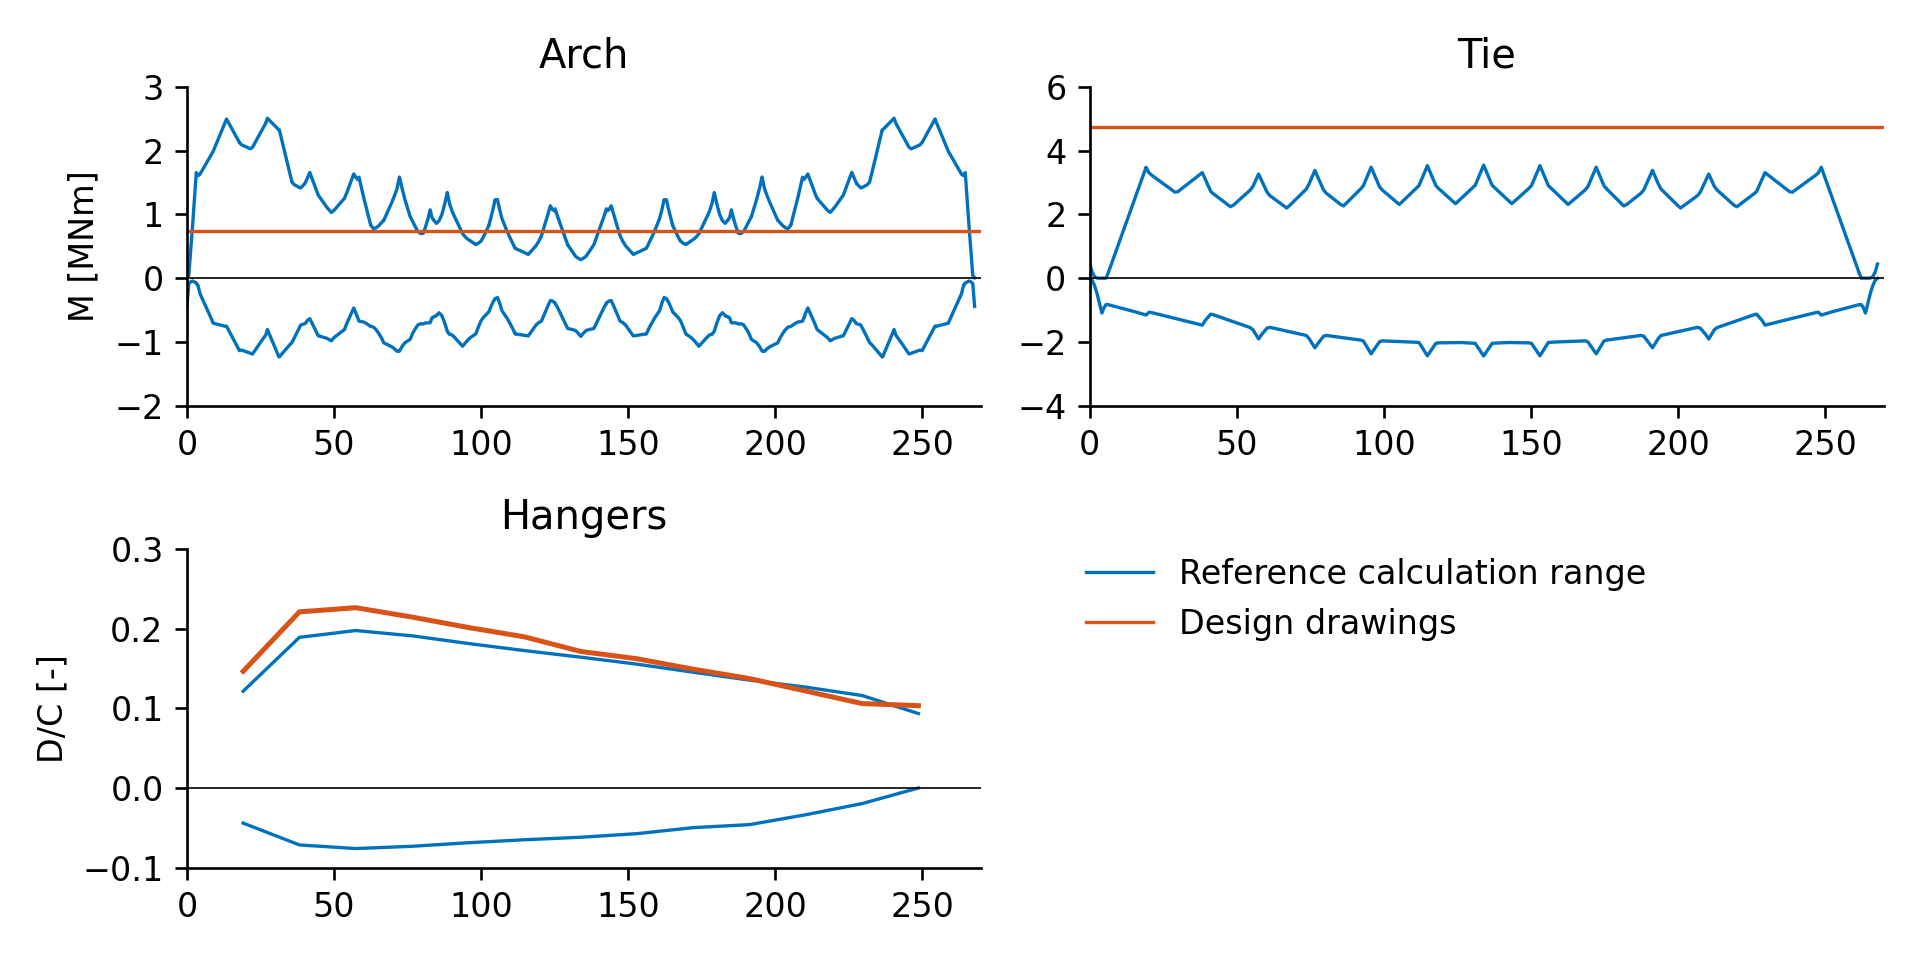
\includegraphics[width=0.8\textwidth]{calculations/Base case/Live load.png}
    \caption{Permanent internal forces of the base case and comparison to the drawings}
    \label{fig:base_case_permanent}
\end{figure}
and compared to the drawings.
